\problemname{Danska}

\noindent

Boschua ska flytta till Lund för att studera vid LTH. 
Du har fått reda på att Lund ligger i Skåne, och nu är du orolig att Boschua ska börja låta dansk.

För att förhindra detta vill du visa Boschua hur många ord som inte alls låter danska. 
Enligt dig låter ett ord danskt om det innehåller minst ett ord från den danska ordboken. 
Tyvärr äger du inte den officiella danska ordboken, men den gamla ordboken du hittade i källaren får duga.

Exempelvis, anta att orboken endast innehåller ordet \texttt{knallert}. Då anser du att ordet \texttt{hus\textbf{knallert}rumma}
låter danskt eftersom det innehåller ordet knallert. Däremot anser du att ordet \texttt{\textbf{knaller}un\textbf{t}} \textbf{inte} låter
danskt eftersom det inte innehåller \texttt{knallert}.
\begin{figure}[h]
  \centering
  \begin{minipage}{0.45\textwidth}
    \centering
    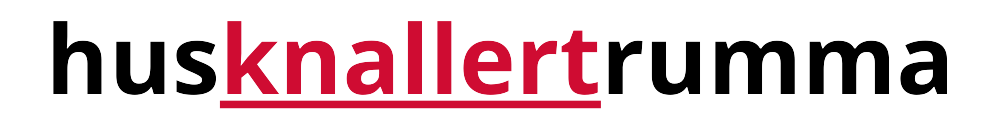
\includegraphics[scale=0.7]{danska-knallert.png}
    \caption{Ordet \texttt{husknallertrumma} låter danskt.}
  \end{minipage}\hfill
  \begin{minipage}{0.45\textwidth}
    \centering
    
\includegraphics[scale=0.7]{knallerunt.png}
    \caption{Ordet \texttt{knallerunt} låter inte danskt.}
  \end{minipage}
\end{figure}

Du inser snabbt att det finns för många ord som inte låter danska för att skriva ner dem alla.
Därför tänker du att det räcker med att räkna antalet ord som inte låter danska och berätta det för Boschua.
Även detta visar sig vara svårt, eftersom det finns så många ord som inte låter danska.

Till slut nöjer du dig med att räkna antalet ord som består av endast små engelska bokstäver
\texttt{a}-\texttt{z}, har exakt $N$ bokstäver och inte låter danska. Ett ord låter för danskt ifall ordet innehåller minst ett ord från ordboken som en delsträng.


\section*{Indata}
Den första raden i indatan innehåller heltalen $N$ ($1 \le N \le 100$) och $M$ ($0 \le M \le 150$),
längden på orden vi betraktar och antalet ord i ordboken.

Därefter följer $M$ rader, där varje rad innehåller ett ord från ordboken. Alla dessa orden har längd som mest $N$
och består av bokstäver \texttt{a}-\texttt{z}. Alla dessa orden är dessutom unika.


\section*{Utdata}
Skriv ut antalet ord av längd $N$ som inte låter för danskt. Eftersom detta talet kan bli väldigt stort,
skriv ut det \href{https://en.wikipedia.org/wiki/Modulo}{modulo} $10^9+7$. 

\section*{Poängsättning}
Din lösning kommer att testas på en mängd testfallsgrupper.
För att få poäng för en grupp så måste du klara alla testfall i gruppen.

\noindent
\begin{tabular}{| l | l | p{12cm} |}
  \hline
  \textbf{Grupp} & \textbf{Poäng} & \textbf{Gränser} \\ \hline
  $1$    & $10$       & $M = 0$ \\ \hline
  $2$    & $13$       & $N \leq 3, M \leq 10$ \\ \hline
  $3$    & $23$       & $M = 1$ \\ \hline
  $4$    & $32$       & $N, M \leq 50$ \\ \hline
  $5$    & $22$       & Inga ytterligare begränsningar. \\ \hline
\end{tabular}

\section*{Förklaring av exempelfall}
I första fallet finns det $26^3$ olika ord. Eftersom den Danska ordboken är tom i detta fallet förbjuds inga av dessa.
